El sistema que se ha planteado ha sido diseñado mediante la siguiente lista de componentes:
\begin{enumerate}
  \item Tecnologías de lado de cliente
  \item Tecnologías de lado de servidor
  \item Control de versiones
  \item Gestión de paquetes
  \item Pruebas unitarias
  \item Pruebas de integración
  \item Pruebas funcionales
  \item Gestor de Base de Datos
  \item Capa de datos
  \item Integración contínua
\end{enumerate}

La figura \cref{fig:architecture} muestra dónde está cada componente y cómo se relaciona con los demás. Por un lado, en la máquina de desarrollo, se podrían encontrar las tecnologías de lado de cliente y servidor (Aplicación y gls{api}), las tecnologías de base de datos y capa de datos y todas las tecnologías de pruebas. La única que quedaría fuera de la máquina de desarrollo es la integración contínua. Además, el entorno de desarrollo cuenta con tecnología de linting, que permite restringir las subidas de código siempre que este no cumpla normativas de limpieza y coherencia.

\begin{figure}
  \centering
  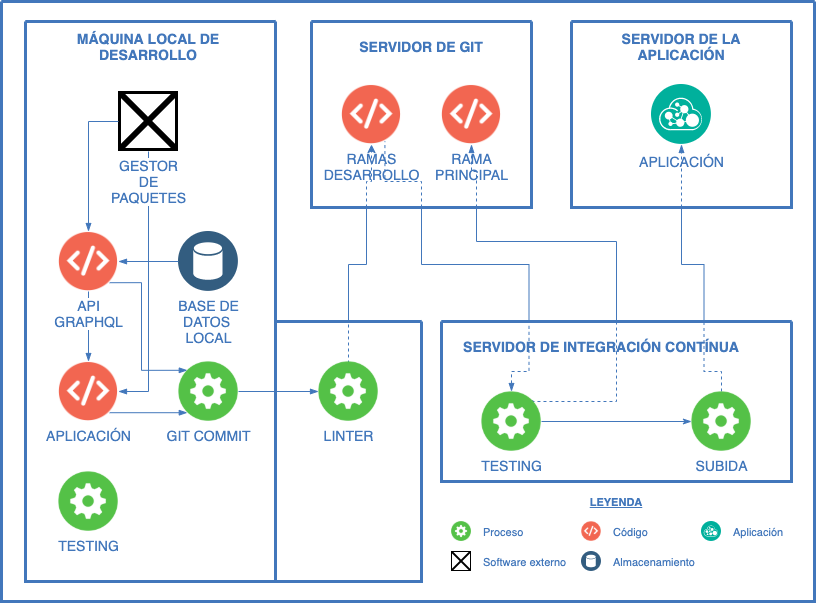
\includegraphics[width=\textwidth]{architecture.png}
  \caption{React Rocket Generator - Architecture}
  \label{fig:architecture}
\end{figure}

Una vez el código cumple los estándares propuestos por el linter y se sube a un repositorio mediante herramientas de control de versiones, se inicia un procedimiento automático descrito en el capítulo de \nameref{section:ci-cd-flow}. En este procedimiento, se utiliza una entidad llamada servidor de integración contínua, que es la responsable de que el flujo se cumpla. En esta entidad vuelven a estar visibles todas tecnologías de pruebas. La máquina de desarrollo tiene acceso a las tecnologías de pruebas como herramienta de desarrollo. Sin embargo, la máquina de integración contínua tiene acceso a estas tecnologías como parte del flujo de integración contínua, y si estás pruebas no son satisfechas, el código no se puede publicar ni en la rama principal ni en el servidor de la aplicación.

Por último, se encuentra el propio servidor de la aplicación, que contiene una versión comprimida del código, junto con la base de datos y la gls{api}. Este servidor es una entidad más compleja, dado que pueden ser varios servidores con un balanceador de carga. Es por eso que ese servidor no entra dentro del marco de desarrollo que se propone y se ha utilizado un icono distinto para representar toda esta complejidad. Cabe destacar que el servidor de integracón contínua y el de la aplicación pueden ser la misma máquina. Sin embargo, este no es el caso habitual y por eso se han marcado como entidades distintas.

Todo el marco está diseñado para que todo lo que hay en la máquina local sea automáticamente configurado mediante una serie de preguntas sencillas. Sin embargo, todo lo que corresponde a las otras máquinas pueden requerir configuración manual. El marco dispone de guías paso por paso para poder configurar todas las conexiones e integraciones descritas en la figura, así como los ficheros de configuración que alimentan el servidor de integración contínua. Todo esto queda explicado más adelante en detalle.

Cabe destacar que este trabajo parte de la premisa de que el marco es solo una propuesta inicial y que, tal y como se explica en el capítulo \nameref{chap:further-steps}, es una propuesta preparada para su expansión.
